\section{Patterns 2 - GoF Observer}

\subsection{Fokuspunkter}

\begin{itemize}
	\item Redegør for, hvad et Software Design Pattern er.
	\item Redegør for opbygningen af GoF Observer.
	\item Sammenlign de forskellige varianter, af GoF Observer - hvilken vil du anvende hvornår?
	\item Redegør for, hvordan anvendelsen af GoF Observer fremmer godt software design.
	\item Redegør for fordele og ulemper ved anvendelsen af GoF Observer.
	\item Redegør for, hvilke(t) SOLID-princip(per) du mener anvendelsen af GoF Observer undersøtter.
\end{itemize}

\subsection{Hvad er et Software pattern?}

\derp

\subsection{Redegør for opbygningen af GoF Observer}
\textit{"Define a one-to-many dependency between objects so that when one object changes state, all its dependents are notified and updated automatically"}\\

Opbygningen kan ses på figur~\ref{fig:observer_classdiagram} side \pageref{fig:observer_classdiagram}, som viser et klassediagram for opbygning af dette pattern.

\begin{figure}[h]
	\centering
	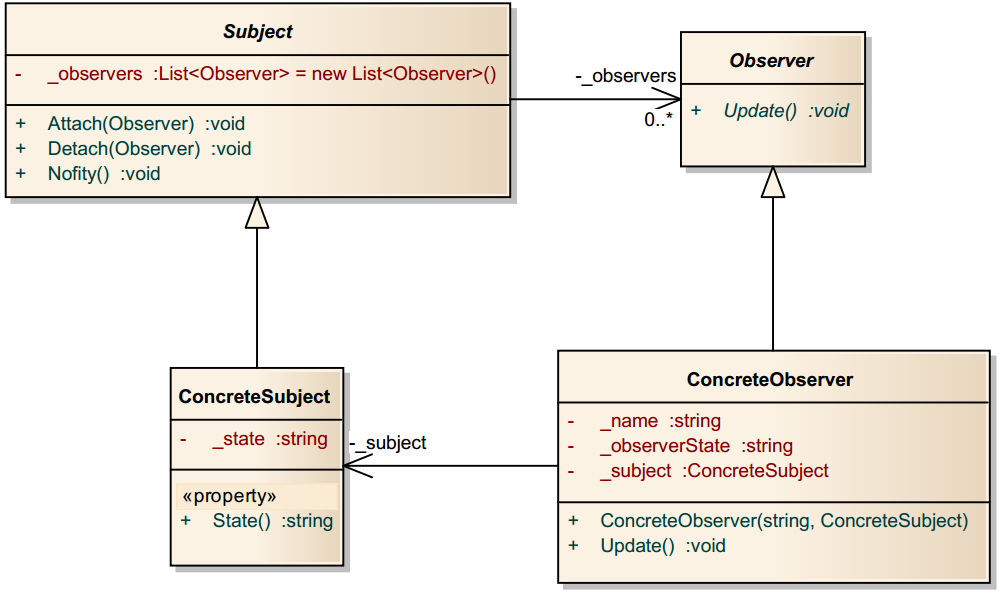
\includegraphics[width=\linewidth]{figs/observer_classdiagram}
	\caption[GoF Observer klassediagram]{Klassediagram som viser GoF Observers opbygning.}
	\label{fig:observer_classdiagram}
\end{figure}


\subsection{Sammenlign de forskellige varianter, af GoF Observer - hvilken vil du anvende hvornår?}

\subsubsection{Many observer to many subjects}
Hvis vi har flere observers som vil observere mere end ét subject objekt, er det ikke nok at \textit{Notify()} om ændringen. I sådant et tilfælde vil det også være nødvendigt at gøre opmærksom på hvilket subject, som ændringen er sket i.

\subsubsection{Who triggers the update?}
Hvis subjectet opdateres meget ofte og vil resultere i unødvendige ændringer af observeren, vil det være bedre om observeren stod for at \textit{trigge} opdateringen.

\subsubsection{Making sure the subject state is self-consistent}
Det er vigtigt at vi ikke kalder \textit{Notify()} funktionen før vores \textit{state} faktisk er opdateret. En løsning er beskrevet på denne side \url{http://www.oodesign.com/observer-pattern.html} og går ud på at lave en template for kaldet, som også kan ses herunder:

\begin{lstlisting}
public void final updateState(int increment)
{
	doUpdateState(increment);
	notifyObservers();
}

public void doUpdateState(int increment)
{
	state = state + increment;		
}
\end{lstlisting}

I dette tilfælde vil vores \textit{ConcreteSubject} bare skulle \textbf{override} \textit{doUpdateState(int)} funktionen og ikke skulle tænke på at kalde \textit{Notify()} på det rigtige tidspunkt.

\subsection{Redegør for, hvordan anvendelsen af GoF Observer fremmer godt software design}

\begin{itemize}
	\item Lav kobling.
	\item Let at udvide.
\end{itemize}

\subsection{Redegør for fordele og ulemper ved anvendelsen af GoF Observer}

\paragraph{Fordele}
Gør det muligt for klasser at reagere på ændringer i en anden klasse uden at koble dem for hoardt.

\paragraph{Ulemper}
Kan give anledning til \textit{memory leaks}. Fordi den simple implementering kræver explicit \textit{registering} og \textit{\textbf{de}registering}. Dette koblet med at \textit{Subject}-klassen har en \textit{strong reference}\footnote{Se wiki om weak reference:\\ \url{https://en.wikipedia.org/wiki/Weak_reference}} til de observers, som kan holde dem unødigt i live.\\
Dette kan dog undgås ved at bruge en \textit{weak-reference}, således at Subject's reference til observeren ikke beskytter mod garbage collectoren hvis det er den eneste.

\subsection{Redegør for, hvilke(t) SOLID-princip(per) du mener anvendelsen af GoF Observer undersøtter}

\begin{itemize}
	\item SRP.\\
	Ikke relevant. Alternativt er den overholdt da klasserne kun har én grund til at ændre sig.
	\item OCP.\\
	Overholdt da vi let vil kunne tilføje flere observers uden at skulle ændre i subject eller anden kode.
	\item LSP.\\
	Brud(?), da man ikke kan udskifte de nedarvede klasser med deres parent.\todo{relevant? Det er jo ikke meningen at dette overhovedet skal kunne gøres?}
	\item ISP.\\
	Overholdt(?), ikke lavet med interface i vores eksempel. Hvis det var gjort med interfaces ville disse være små og lette. 
	\item DIP.\\
	Ikke relevant, da \todo{how to explain?}
\end{itemize}